\section{Example Tests}
\paragraph{}
During the development of the Framework, many tests have been developed, to both test the capabilities of the framework, and to be used in real studies. Following some of those scenes are described.


\subsection[Influence of continuous depth]{Pilot Study: Influence of continuous depth on fatigue}
\paragraph{}
Objective of the study is to quantify the effect of a continuous depth element on the time it takes participants to focus objects at various depths, and the change in refocus time with the progression of the experiment.

\begin{center}
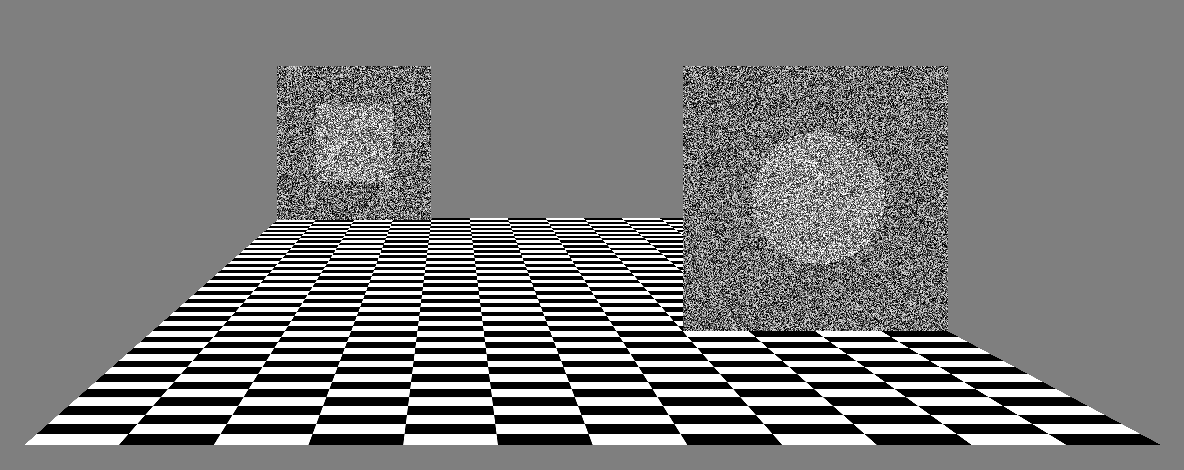
\includegraphics[width=7.5cm]{media/pilotFatigue.png}
\end{center}

\paragraph{}
The test stimulus consists of a grey background (50\% grey), a continuous depth element (plane, checkerboard pattern, averaging in 50\% grey) and two random dot targets (approximately 50\% grey).
The targets show a shape which is either convex (coming out of the screen), or concave (going into the screen).
For the encoding details see section \ref{RDS}. The random pattern consists of eight shades of grey, of which the dark seven are used for the background, and the light seven for the foreground.

The random dot targets are resting on the plane, and border to either the left or the right border.
Each target can be at  one of three depth locations, at a separation of \unit{-3.1}{°}, \unit{0}{°} (parallax plane) and \unit{3.1}{°}.

The image is back-projected on a screen by two projectors through circular polarisation filters. The image height is \unit{0.7}{m}, it's width is \unit{1.17}{m}. The participant's head is at \unit{1}{m} distance of the screen, and observes the screen with polarised filter goggles. The room is dark.

\todo{Write about independent/dependent variables, logging}

\todo{Write about randomness of various things}

\todo{Write about ...}